\mathversion{bold}
\chapter{Cloning of the $\sigmaup$ Subunits}
\mathversion{normal}

\section{Introduction}
\label{chap3:intro}
%Several techniques have been employed to clone
%subunits of RNA polymerase from different species of bacteria.
%Sequence conservation led to the development of specific probe,
%PCR primers or even full length gene has been used for
%heterologous cloning. Functional conservation enabled cloning by
%functional complementation.

Ever since the cloning of \emph{E. coli rpoD} \citep{Burton1981},
enumerable $\sigmaup$ genes have been cloned from several
bacterial species. A specific oligomer of 29 bases named
``\textit{rpoD}-box'' \citep{Tanaka1988} had been used,
traditionally, to clone $\sigmaup$\su{70} family homologs from
various species, Gram-positive and Gram-negative bacteria, and
even cyanobacteria. A stretch of amino acids (\seq{TYATWWIRQA})
was found to be conserved between region 2.3 and 2.4 of all known
$\sigmaup$\su{70} family members including, \textit{rpoH} and
\textit{rpoS}\@. The oligonucleotide designed from this sequence
(5$'$G\-C\-T\-T\-G\-I\-C\-I\-I\-A\-T\-C\-C\-A\-C\-C\-A\-I\-G\-T\-I\-G\-C\-I\-T\-A\-I\-G\-T3$'$)
was used to probe and clone several $\sigmaup$-factors, such as
$\sigmaup$\su{70} of \textit{P. aeruginosa} \citep{Tanaka1991},
$\sigmaup$\su{32} of \textit{P. aeruginosa} \citep{Naczynski1995},
\textit{sigA} of \textit{Chlamydia psittaci}, \textit{hrdA, B, D,
E} from \textit{Streptomyces spp.}\
\citep{Kormanec1992,Tanaka1991b}, \textit{sigA} and \textit{sigB}
of \textit{B. lactofermentum} \citep{Oguiza1996} and several
others.

The sequence conservation in region 2 and 4 of $\sigmaup$\su{70}
family also led to development of PCR primers which were used to
amplify a fragment from the gene. Several $\sigmaup$ factors were
cloned using this method, notably, \textit{rpoD} of
\textit{Chlamydia trachomatis} \citep{Engel1990},
\textit{Bordetella pertussis} \citep{Steffen1997},
\textit{Xanthomonas campestris} \citep{Tseng1997},
\textit{Rhizobium spp.}\ \citep{Rushing1995,Luka1996};
\textit{sigF} from \textit{Mycobacterium tuberculosis}
\citep{DeMaio1996}.

Full-length gene from one species was also used as heterologous
probe to clone $\sigmaup$ factor from another species\@.
\textit{rpoD} from \textit{P. putida} was cloned using \textit{P.
aeruginosa rpoD} gene as probe \citep{Fujita1995}.
\textit{Heliobacillius mobilis sigA} was cloned using
\textit{Synechococcus sp.}\ strain PCC7002 \textit{sigB} as probe.
\textit{Thermotoga maritima} and \textit{Rhodobacter sphaeroides
sigA} were cloned using \textit{H. mobilis sigA} as probe
\citep{Gruber1997}.

The close structural and functional resemblance was also used to
clone several $\sigmaup$-factors using functional complementation.
\textit{P. aeruginosa rpoH} was cloned making use of the fact the
bacteriophage $\lambda$ is unable to form plaque on \textit{E.
coli} strains lacking functional \textit{rpoH}
\citep{Benvenisti1995}. \textit{Pseudomonas putida} KT2440
\textit{rpoS} gene was cloned using \textit{E. coli} strain ZK918
which lacks \textit{rpoS} and contains a fusion of
\textit{bolAp$_{1}$} promoter with \textit{lacZ}. Upon mobilizing
a genomic library of \textit{P. putida} in ZK918, functional
\textit{rpoS} was cloned based on the fact that \textit{lacZ}
expression is more in ZK918 containing \textit{rpoS} gene
\citep{Ramos1998}.

The other RNA polymerase subunits, $\alphaup$, $\betaup$ and
$\betaup'$ were cloned from several species of bacteria taking
advantage of the sequence conservation. The same strategy was used
for cloning several other $\sigmaup$ factors including
$\sigmaup$\su{N} and $\sigmaup$\su{E} genes.

In this study three strategies were followed to clone \e{rpoD} and
\emph{rpoS} of \bact{Ps} Lz4W:

\begin{enumerate}[a)]

\item Design of oligomeric probes and primers based upon the most
conserved regions of the $\sigmaup$ family and use them as probe
in screening genomic libraries, or use them as primers for PCR
amplification.

\item Heterologous full-length gene as probe to screen genomic
libraries.

\item Functional complementation of \bact{Ec} mutants.
\end{enumerate}

As will be shown in this chapter, a partial ORF, coding for
putative \emph{rpoD} (\emph{rpoD}$_{Lz4W}$) and the full-length
ORF coding for the putative \emph{rpoS} (\lzsig{}) was cloned from
Lz4W by screening genomic libraries, using a heterologous gene and
PCR amplified fragments of corresponding genes as probes. The
possibility of cloning other RNA polymerase subunits and
\emph{rpoH}, the heat-shock $\sigmaup$ factor in Lz4W, were also
investigated using heterologous probes.

\section{Results}

\subsection{Cloning of \emph{rpoD} and \emph{rpoS} homologs}

\subsubsection{Use of ``\emph{rpoD}'' box probe}
In the first attempt to clone the \e{rpoD} and \e{rpoS} of Lz4W,
one degenerate (Probe2 in Figure~\ref{chap3:rpod_box}C) and
another more specific oligomer (Probe1 in
Figure~\ref{chap3:rpod_box}C) of 29 bases long, were synthesized
as described in \citet{Tanaka1988}. The degenerate version of this
oligomer named \textit{``rpoD box''}, designed from the most
conserved amino acids (TYATWWIRQA) in region 2.3/2.4 of
$\sigmaup$\su{70} family of $\sigmaup$ factors had earlier been
used to clone various $\sigmaup$ factors (see Section
\ref{chap3:intro}). The strategy of the design of these oligomers
is shown in Figure \ref{chap3:rpod_box}.

\begin{figure}[tbp]
\centering
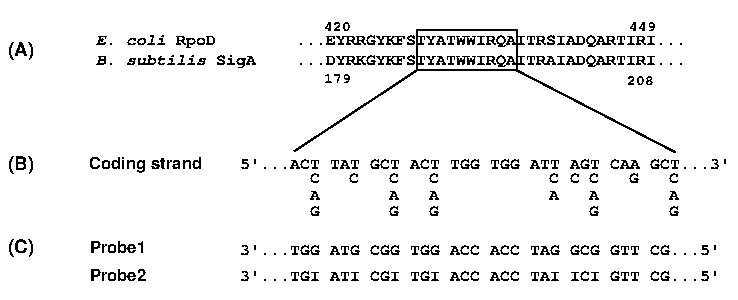
\includegraphics{figures/chap3_rpod_box}
\caption[Design of ``\textit{rpoD} box'' probe]{Design of
``\textit{rpoD} box'' probe. \textbf{(A)} Alignment of the
\textit{E. coli} RpoD and \textit{B. subtilis} SigA. The numbers
above the \textit{E. coli} sequence and the below \textit{B.
subtilis} sequence are the amino acid residues. The boxed amino
acids denote the ``\textit{rpoD} box''. \textbf{(B)} The deduced
coding strand showing the possible nucleotide sequence.
\textbf{(C)} shows the synthesized oligomers. Probe1 is a
"guessmer", synthesized considering the high GC codon bias in
\emph{Pseudomonas}. Note the use of inosine for degenerate
positions in Probe2. Modified and redrawn from
\citet{Tanaka1988}.} \label{chap3:rpod_box}
\end{figure}

Earlier studies in our laboratory had identified and cloned a
genomic fragment from Lz4W using Probe1 in
Figure~\ref{chap3:rpod_box}C. The plasmid was sequenced using
subcloning of the restriction fragments in pUC19. It contained a
\U{5.2}{kb} insert spanning partial \emph{pot} and \emph{pho}
operon with no apparent sequence similarity with any known
$\sigmaup$ gene (data not shown).

In order to circumvent the problem associated with the
non-specificity of the Probe1, the second degenerate probe, Probe2
was synthesized (Figure~\ref{chap3:rpod_box}C). Probe2, when used
in Southern hybridization analysis, detected two bands in genomic
DNA digested with \emph{Pst}I (Lane 1 in
Figure~\ref{chap3:rpod_box_southern}). To clone these two DNA
fragments a  partial genomic library was made by eluting the DNA
from these bands and ligating the eluted DNA to pUC19. Even after
repeated screening, we failed to detect any positive clone in the
library generated from the DNA of the upper band. However, a
positive clone was detected in the library, made using DNA from
the lower band. Upon sequencing the plasmid, it was found that the
\U{2}{kb} insert of the plasmid contains two ORFs very similar in
sequence to that of \emph{trk}, \emph{fmu} sequences of \emph{E.
coli} (data not shown), with no apparent sequence similarity to
any known $\sigmaup$ factor. Nevertheless, another set of
libraries were made in pBluescriptII KS+, using the DNA eluted
from the same positive bands. Once again the probe failed to
detect any positive clone in library made from the DNA of the
upper band. On screening the library made with the DNA eluted from
the lower band, the probe again detected the false positive clone
containing \emph{trk} and \emph{fmu}, for the second time. The
reason why the Probe2 binds to this DNA fragment is still
unexplainable.

\begin{figure}[tbp]
\centering
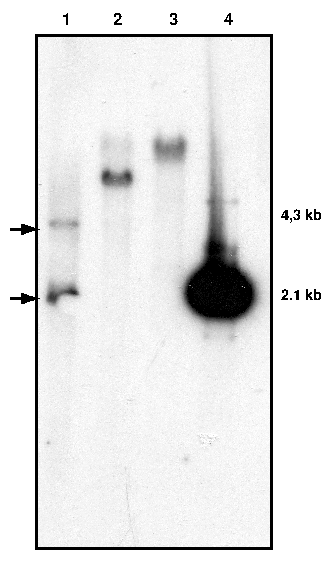
\includegraphics{figures/chap3_rpod_box_southern}
\caption[Genomic Southern blot analysis using ``\emph{rpoD} box''
probe]{%
    Genomic Southern hybridization analysis using ``\emph{rpoD} box''
    probe. Probe2 in Figure~\ref{chap3:rpod_box}C was used to
    probe genomic DNA of Lz4W digested with several enzymes. The
    positive bands on \emph{Pst}I digested DNA was marked with
    arrows on the left side. Right side shows the calculated
    marker positions. The numbers on the top shows the lane
    numbers. Lane 1, Lz4W genomic DNA digested with \emph{Pst}I;
    lane2, Lz4W genomic DNA digested with \emph{Eco}RI; lane 3,
    Lz4W genomic DNA digested with \emph{Xho}I; lane 4, plasmid
    pGEMD~\citep{Igarashi1991} digested with \emph{Hin}dIII which
    contains the full-length \emph{rpoD} gene of \emph{E. coli},
    loaded as positive control.}
\label{chap3:rpod_box_southern}
\end{figure}

\subsubsection{Full-length genes as heterologous probes}

Having failed to detect any true positive clone with the
``\e{rpoD} box'' oligomeric probe, an alternative strategy was
considered. The suitability of the full length \emph{rpoD} of
\emph{E. coli} and \emph{P. aeruginosa} gene as heterologous
probes was tested in genomic Southern blot analysis. The
\U{2.1}{kb} \emph{Hin}dIII fragment containing the full-length
\emph{rpoD} of \emph{E. coli} from plasmid
pGEMD~\citep{Igarashi1991} and \U{2.3}{kb} \emph{Pst}I insert from
plasmid pASB3~\citep{Tanaka1991} containing the full-length
\emph{rpoD} of \emph{P. aeruginosa} were used. Both these genes,
when used as probes for genomic Southern hybridization analysis,
bound poorly to the Lz4W genomic DNA under high stringency.

\emph{P. aeruginosa rpoS} gene, on the other hand, bound strongly
to Lz4W genomic DNA, as shown in the
Figure~\ref{chap3:pdb18r_southern}. The \U{$\sim$1.8}{kb}
\emph{Kpn}I--\emph{Hin}dIII insert from the plasmid
pDB18R~\citep{Fujita1994}, spanning the full-length \emph{rpoS} of
\emph{P. aeruginosa}, was used as probe in Southern blot analysis.
The position of the positive bands in the lane containing
\emph{Pst}I digested DNA (lane 1 in
Figure~\ref{chap3:pdb18r_southern}B) was identical to what was
observed with ``\emph{rpoD} box'' probe (lane 1 in
Figure~\ref{chap3:rpod_box_southern}). This indicated that the
lower band detected by ``\emph{rpoD} box'' probe in \emph{Pst}I
digested genomic DNA of Lz4W was presumably the \emph{rpoS}
homolog.

\begin{figure}[tbp]
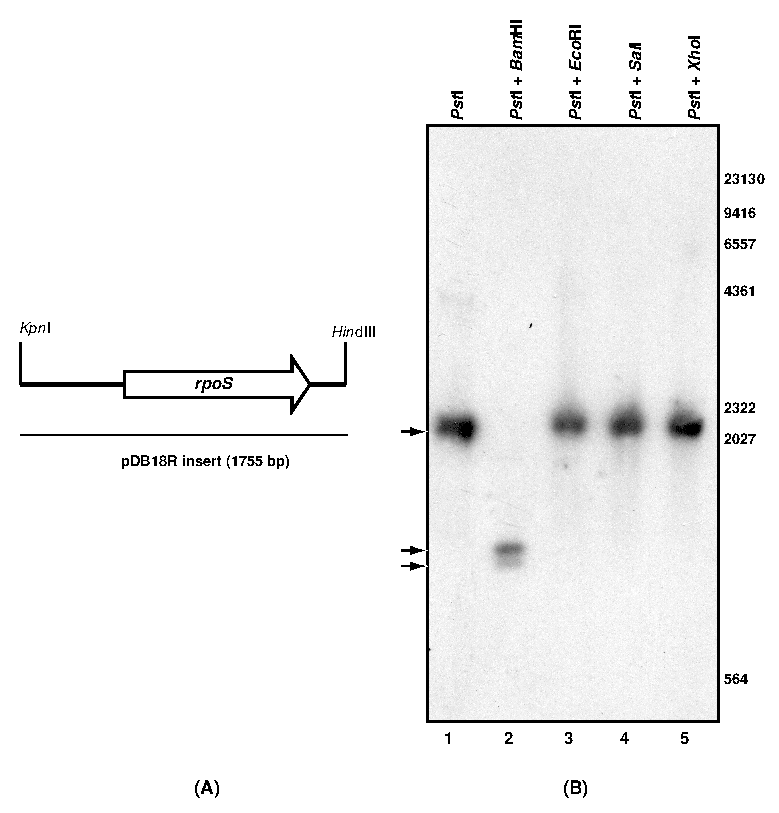
\includegraphics{figures/chap3_pdb18r_southern}
\caption[Genomic Southern blot analysis using \emph{P. aeruginosa
rpoS} as probe]{%
    Genomic Southern hybridization analysis using \emph{P. aeruginosa rpoS}
    as probe. \textbf{(A)} shows the probe used. The \U{$\sim$1.8}{kb} \emph{Kpn}I--\emph{Hin}dIII insert from
    plasmid pDB18R~\citep{Fujita1994} was used to probe the genomic DNA of Lz4W digested with various enzymes.
    The line below the map shows the span of the probe used. \textbf{(B)} shows the autoradiogram. Numbers along the right side
indicate the markers in base-pairs. The positive bands are shown
with arrows on the left. Approximately \mug{3} digested DNA was
loaded in each lane. The enzymes used are indicated on the top of
each lane and numbers below each lane show the lane numbers. Lane
1, \emph{Pst}I; lane 2, \emph{Pst}I and \emph{Bam}HI; lane 3,
\emph{Pst}I and \emph{Eco}RI; lane 4, \emph{Pst}I and \emph{Sal}I;
lane 5, \emph{Pst}I and \emph{Xho}I.}
\label{chap3:pdb18r_southern}
\end{figure}

\subsubsection{Functional complementation of \emph{E. coli rpoS}
mutant}

With the idea that the lower band (\U{$\sim$2}{kb}) detected by
the ``\emph{rpoD} box'' in \emph{Pst}I digested genomic DNA of
Lz4W was probably \emph{rpoS} homolog, an attempt was made to
clone the gene by functional complementation of \emph{E. coli
rpoS} mutant. The strategy was to make use of a strain of \emph{E.
coli} called ZK918~\citep[see Table~\ref{ecolistrains} on page
\pageref{ecolistrains} for genotype]{Bohannon1991}. This strain is
\emph{rpoS}-deficient due to a deletional insertion generated with
a \emph{rpoS}::Km fusion. The strain also carries a chromosomal
insertion of a transcriptional fusion of \emph{bolAp1} promoter to
the \emph{lacZ} at the \emph{bolA} locus. Because
\emph{bolAp}$_{1}$ promoter is \emph{rpoS}-dependent, the
phenotype of the strain was reported to be RpoS\su{$-$}
LacZ\su{$-$}~\citep{Bohannon1991,Ramos1998}. The strain had been
used earlier to clone \emph{rpoS} homolog from \emph{P. putida}
KT2440~\citep{Ramos1998}.

A partial genomic library was made with the DNA eluted from the
lower band (lane 1 in Figure~\ref{chap3:rpod_box_southern}) in
pBluescriptII KS+ vector and electroporated into ZK918. An aliquot
of the cells was plated on kanamycin, ampicillin and X-gal
containing LB agar plates without any treatment. Since \emph{rpoS}
is known to confer acid-resistance, \emph{rpoS} containing cells
were enriched by first treating the cells with acid, and then
neutralizing, before plating on selection plates. For acid
treatment, \mul{200} of transformed cells in LB was treated with
\mul{10} of \U{1}{N} HCl for \U{30}{min}. The suspension was then
neutralized by addition of \mul{10} of \U{1}{N} NaOH before
plating on ampicillin, kanamycin and X-gal containing plates. It
was observed that ZK918 cells had too high background
$\betaup$-galactosidase activity to visually distinguish between
RpoS\su{$-$} and RpoS\su{$+$} cells. An attempt was made to select
the cells with higher $\betaup$-galactosidase activity by plating
the cells in lactose minimal media containing ampicillin and
kanamycin. But even on these plates the \emph{rpoS} harboring
cells were indistinguishable from the background control cells.

\subsubsection{Use of degenerate primers}
Due to the failures in strategies described above, degenerate PCR
primers were designed from the most conserved regions of
$\sigmaup$\su{70} family as shown in Figure~\ref{chap3:primers}.
The forward primers, RPODFP1 and RPODFP2, were designed from
region 2.3/2.4 and reverse primers, RPODRP1 and RPODRP2, were
designed from region 4.2 (Figure~\ref{chap3:primers}C). The
primers were designed with different level of degeneracies. Both
these primers when used in PCR with Lz4W genomic DNA as template,
amplified a \U{400}{bp} DNA fragment. The amplified DNA was
purified from the gel and cloned into TA cloning vector pGEM-T.
Four positive clones carrying insert, were detected, and named as
pT1, pT6, pT7, and pT9. The inserts in these clones were named T1,
T6, T7, and T9 respectively. All these inserts were sequenced and
a careful examination of the sequence and database search using
BLAST revealed that the T1 is a fragment of \emph{rpoS}, and T7 is
a fragment of \emph{rpoD}. T6 and T9 were generated by fusion of
\emph{rpoS} and \emph{rpoD} DNA fragments as PCR artifacts. The
BLAST result of T1 and T7 are summarised in
Table~\ref{chap3:blast_summary}.

\begin{sidewaysfigure}[tbp]
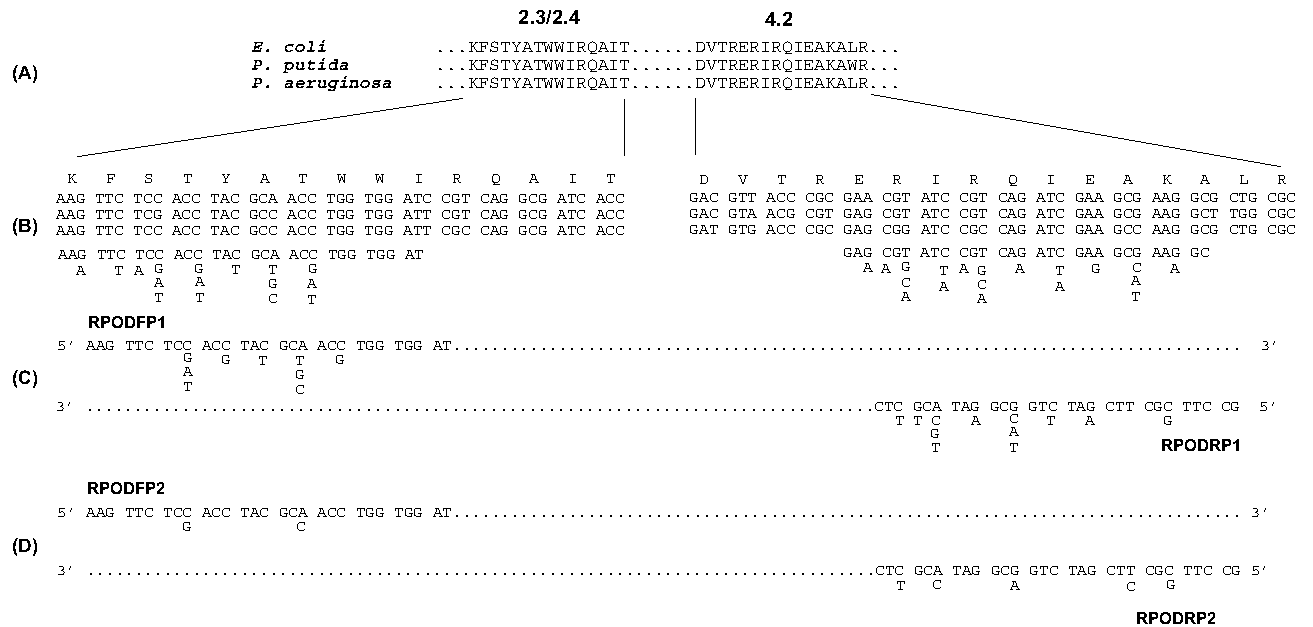
\includegraphics{figures/chap3_1}
\caption[Primer design strategy]{Primer design strategy. (A)
\emph{E.coli} (GenBank accession  J01687), \emph{P. putida}
(GenBank accession D30045) and \emph{P. aeruginosa} (GenBank
accession D90118) \emph{rpoD} sequences were aligned. Only the
regions used to design primers (from 2.3/2.4 and 4.2) are shown.
(B) The corresponding nucleotide sequence alignment is shown with
the bottom most track showing the degeneracy at the third codon
position. (C) and (D) show the pairs of degenerate primers
designed. The degeneracy was reduced considering the high GC
content of \emph{Pseudomonas} sp. genome.} \label{chap3:primers}
\end{sidewaysfigure}

\begin{table}[tbp]
\begin{minipage}[c]{\textwidth}
\renewcommand{\footnoterule}{}
\caption[Summary of BLASTX statistics for PCR amplified
\emph{rpoD} and \emph{rpoS} fragments]{Summary of BLASTX
statistics for PCR amplified \emph{rpoS} and \emph{rpoD}
fragments\protect\footnote{The top five BLASTX hit statistics are
shown for each case}} \label{chap3:blast_summary} \centering
\begin{small}
\begin{tabular}{llccc}\toprule
\textbf{Organism} & \textbf{Gene} & \textbf{Accession} &
\textbf{Score} & \textbf{E-value}\\\midrule\addlinespace
\multicolumn{5}{l}{\textbf{Fragment T1}}\\ \emph{Pseudomonas
tolaasii} & \emph{rpoS} & AB006073 & 114 & $3
\times{}10^{-43}$ \\
\emph{Pseudomonas fluorescens} & \emph{rpoS} & U34203 & 115 &
$4\times{}10^{-43}$ \\
\emph{Pseudomonas syringae} pv. tomato & \emph{rpoS} & AF061853 &
114  & $8\times{}10^{-43}$ \\
\emph{Pseudomonas putida}& \emph{rpoS} & X91654 &
113 & $2\times{}10^{-42}$\\
\emph{Pseudomonas aeruginosa} & \emph{rpoS} & P45684 & 112 &
$3\times{}10^{-41}$\\\addlinespace \multicolumn{5}{l}{\textbf{Fragment T7}}\\
\emph{Pseudomonas fluorescens} & \emph{rpoD} & P52326 & 189 &
$8\times{}10^{-48}$ \\
\emph{Pseudomonas putida} & \emph{rpoD} & U93292 &  189 &
$8\times{}10^{-48}$ \\
\emph{Pseudomonas tolaasii} & \emph{rpoD} &AJ007830 &  189 &
$8\times{}10^{-48}$ \\
\emph{Pseudomonas aeruginosa} & \emph{rpoD} & P26480 &  188 & $2\times{}10^{-47}$ \\
\emph{Pseudomonas putida} & \emph{rpoD} & P52327 &  186 &
$7\times{}10^{-47}$ \\
\bottomrule
\end{tabular}
\end{small}
\end{minipage}
\end{table}

When used as probe in genomic Southern hybridization analysis, all
these DNA fragments hybridized strongly to Lz4W genomic
DNA(Figure~\ref{chap3:tprobes}). Although T6 is a PCR artifact, it
gave expected Southern pattern (lanes 2--6 in
Figure~\ref{chap3:tprobes}). T1 being \emph{rpoS} fragment, bound
to the lower \emph{Pst}I band (lane 1 in
Figure~\ref{chap3:tprobes}) and T7 bound to the upper band (lane 7
in Figure~\ref{chap3:tprobes}). This result also confirmed that
the \U{$\sim$4}{kb} \emph{Pst}I band indeed contained \emph{rpoD},
and the \U{$\sim$2}{kb} \emph{Pst}I band contained \emph{rpoS}.
The result also indicated that there was a \emph{Bam}HI site
within both \emph{rpoD} and \emph{rpoS} (lane 3), and that  a
\emph{Sal}I site exists within \emph{rpoD} (lane 5 in
Figure~\ref{chap3:tprobes}).

\begin{figure}[tbp]
\centering
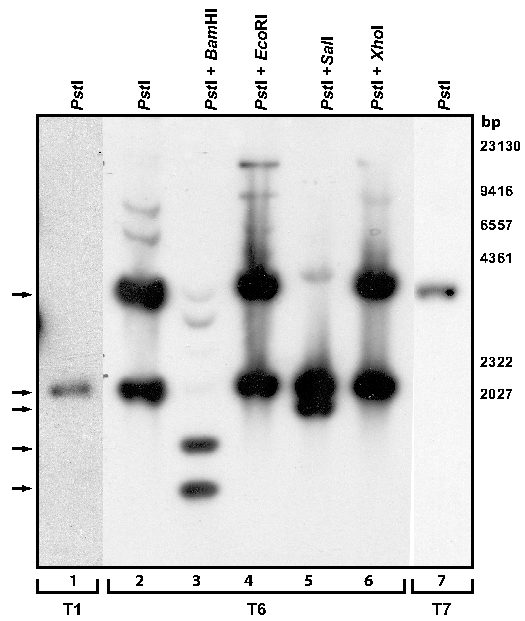
\includegraphics{figures/chap3_tprobe_southern.pdf}
\caption[Southern blot analysis using PCR-amplified \emph{rpoD}
and \emph{rpoS} fragments]{%
    Southern blot analysis of Lz4W genomic DNA using PCR-amplified \emph{rpoD} and \emph{rpoS}
    fragments. The numbers on the right side indicates the marker
    is base-pairs. The probes used are marked below (for the
    description of the probes, see
    Table~\ref{chap3:blast_summary} and text). The positive bands are indicated by arrows on the left. The enzymes used for digestion of genomic DNA are
    indicated on top. Lane 1, 2 and 7, \emph{Pst}I; lane 3,
    \emph{Pst}I and \emph{Bam}HI; lane 4, \emph{Pst}I and
    \emph{Eco}RI; lane 5, \emph{Pst}I and \emph{Sal}I; lane 6,
    \emph{Pst}I and \emph{Xho}I.}
\label{chap3:tprobes}
\end{figure}

\subsubsection{Complementation of \emph{E. coli rpoD} mutant}

With the indication that the bigger \emph{Pst}I fragment probably
contained \emph{rpoD}, an attempt was made to clone the gene by
functional complementation of \emph{E. coli rpoD} mutant. For
complementation,  a strain of \emph{E. coli} named UQ285 was used,
which harbors a temperature-sensitive \emph{rpoD}
allele~\citep{Isaksson1977}. This strain was unable to grow at
42\dg{} unless complemented by a fully functional \emph{rpoD}\@.
The DNA extracted from the \U{$\sim$4}{kb} region of the gel was
ligated to plasmid pBluescriptII KS+, and electroporated into
UQ285. The transformed cells were plated on LB agar plates
containing ampicillin, and incubated at 42\dg{}. Surprisingly,
there were no complemented clone. This suggested that either the
fragment does not contain the full-length gene of \e{rpoD}, or the
gene was not functional in \bact{Ec}. The inability of Lz4W
\e{rpoD} to complement the functions of \bact{Ec} \e{rpoD} also
could not be ruled out.

To test the idea whether the high-copy number of the vector
pBluescriptII KS+ that was used for complementation was having a
detrimental effect on the cell survival, the complementation
experiment was repeated using a low-copy number vector
pCL1920~\citep{Lerner1990}. Even in this case there was no
complemented clone.

\subsubsection{Cloning of \emph{rpoD} in fragments}

After the failure in cloning the full-length \e{rpoD}, an attempt
was made to clone the gene in separate fragments, taking advantage
of the presence of a single \emph{Sal}I site within the gene.
Following separation of the \emph{Pst}I and \emph{Sal}I digested
genomic DNA on preparative agarose gel, DNA from the \U{2}{kb}
region was extracted and a partial genomic library was made in
pBluescriptII KS+. A positive clone was detected using the T7
probe. The plasmid isolated from this clone, p4A4, was almost
fully sequenced. Database search revealed that it contained a
partial ORF at the \emph{Sal}I end and another partial ORF at the
\emph{Pst}I end. Upon running BLAST against GenBank we found that
the clone contained partial ORF of \emph{rpoD} at the \emph{Sal}I
end. A map of the insert is shown in Figure~\ref{chap3:4a4}A and
the sequence of the partial \emph{rpoD} is shown in
Figure~\ref{chap3:4a4}B. The summary of the BLAST statistics is
shown in Table~\ref{chap3:4a4_blast}. The highest similarity of
the aligned region was with \emph{P. tolaasii} (BLAST positive,
98\%) and with \emph{P. fluorescens} (BLAST positive 98\%).
According to the alignment, the cloned \emph{rpoD}$_{Lz4W}$
started from the codon 314 of \emph{P. tolaasii} \emph{rpoD} and
codon 315 of \emph{P. fluorescens}. The \emph{E. coli rpoD} was
only 89\% (BLAST positives) similar. All similarity scores were
calculated using BLOSUM62 matrix.

\begin{sidewaysfigure}[tbp]
\centering
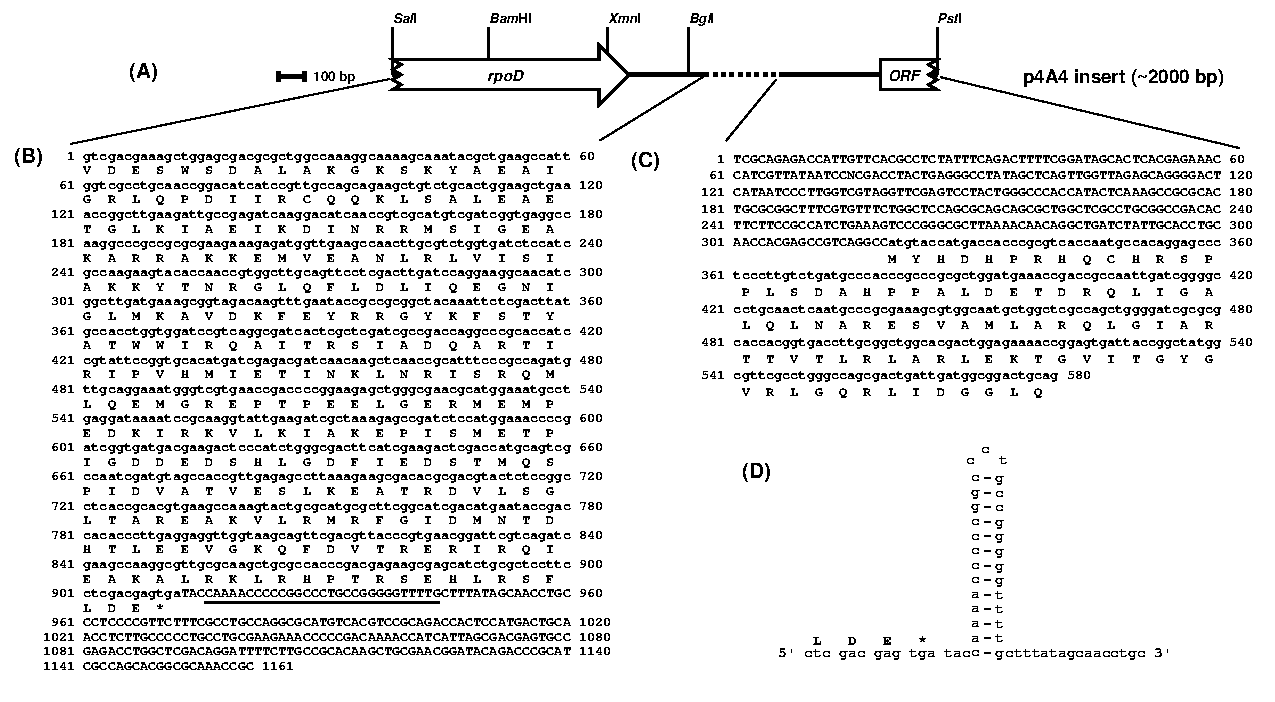
\includegraphics{figures/chap3_4a4}
\caption[\emph{rpoD} homolog of Lz4W]{\textbf{(A)}Schematic
diagram of the insert in p4A4, drawn to  scale. Broken arrows
denote partial ORFs. Dotted line indicates the region not
sequenced. \textbf{(B)} The sequence of the partial \emph{rpoD}
homolog of Lz4W. Translated amino acids are shown below the
sequence. The underlined sequence is $\rhoup$-independent
transcription termination signal. \textbf{(C)} The conserved ORF
downstream of \emph{rpoD}. \textbf{(D)} The $\rhoup$-independent
transcription termination signal downstream of \emph{rpoD} ORF
($\Delta$G $-$24.3 kcal/mol).} \label{chap3:4a4}
\end{sidewaysfigure}

\begin{table}[tbp]
\begin{minipage}[c]{\textwidth}

\renewcommand{\footnoterule}{}
\caption[Summary of BLASTX statistics of
\emph{rpoD}$_{Lz4W}$]{Summary of BLASTX statistics of
\emph{rpoD}$_{Lz4W}$\protect\footnote{The top five BLASTX hit
statistics are shown.}} \label{chap3:4a4_blast}
\begin{narrow}{-1in}{-1in} \centering
\begin{small}
\begin{tabular}{llcccc}\toprule
\textbf{Organism} & \textbf{Gene} &
\multicolumn{1}{p{1.1in}}{\textbf{GenBank or Swiss\-Prot
Accession}\protect\footnote{GenBank accession are prepended with
gb: and SwissProt accession are prepended with sp:.}} &
\textbf{Score} & \textbf{E-value} & \textbf{\%
similarity}\protect\footnote{According to BLOSUM62
matrix.}\\\midrule\addlinespace \emph{Pseudomonas tolaasii} &
\emph{rpoD} & gb:AJ007830
 & 583 & $10^{-165}$ & 98 \\
\emph{Pseudomonas fluorescens} & \emph{rpoD} & sp:P52326
 & 583 &$10^{-43}$ &98\\
\emph{Pseudomonas putida} & \emph{rpoD} & sp:P52327 &
539  & $10^{-152}$ & 93\\
\emph{Pseudomonas aeruginosa} & \emph{rpoD} & sp:P26480 & 538 &
$10^{-152}$ & 94\\
\emph{Shewanella violacea} & \emph{rpoD} & sp:O24744 & 507 &
$10^{-143}$ & 91 \\
%\emph{Salmonella typhimurium} & \emph{rpoD} & sp:P07336 &  499 & $10^{-140}$ & 90 \\
\bottomrule
\end{tabular}
\end{small}
\end{narrow}
\end{minipage}
\end{table}

A putative $\rhoup$-independent transcription termination signal
was also detected (Figure~\ref{chap3:4a4}D) downstream of the
\emph{rpoD} ORF. There was also an ORF with domain structure of a
transcription factor as shown in Figure~\ref{chap3:4a4}C. This ORF
is conserved in large group of proteobacteria including \emph{P.
putida}~(GenBank accession AF302763).

\subsubsection{Cloning of \emph{rpoS}}




For cloning of \e{rpoS}, two types of genomic libraries were used,
a cosmid library and a partial genomic library in plasmid. The
cosmid  genomic library was constructed in cosmid
pLAFR3~\citep{Staskawicz1987} as described in
Section~\ref{chap2:cosmid_library}. A simultaneous screening of
the cosmid library and a partial genomic library in plasmid
pBluescriptII KS+ from the \emph{rpoS} region of \emph{Pst}I
digested genomic DNA, was carried out. A positive clone was
detected in the plasmid library using T1 and the insert from
plasmid pDB18R as probes. The plasmid, named p4C12, contained a
\U{$\sim$2}{kb} \emph{Pst}I insert. By subcloning and direct
sequencing with primers full sequence of the insert was
determined. Upon database search it was found that it contained
the full ORF of \emph{rpoS} and a partial ORF from the upstream
\emph{nlpD} gene. The summary of the BLASTX statistics for
\emph{rpoS}$_{Lz4W}$ is shown in Table~\ref{chap3:4c12_blast}. As
shown in the Table~\ref{chap3:4c12_blast} the closest sequence
similarity was with \emph{P. fluorescens} (BLAST positive score,
80\%). The BLAST positive score was only 75\% with \bact{Ec}
\emph{rpoS}. A schematic diagram of the insert in p4C12 is shown
in Figure~\ref{chap3:4c12_map} and the full sequence is shown is
Figure~\ref{chap3:4c12}.


\begin{table}[tbp]
\begin{minipage}[c]{\textwidth}

\renewcommand{\footnoterule}{}
\caption[Summary of BLASTX statistics of
\emph{rpoS}$_{Lz4W}$]{Summary of BLASTX statistics of
\emph{rpoS}$_{Lz4W}$\protect\footnote{The top five BLASTX hit
statistics are shown.}} \label{chap3:4c12_blast}
\begin{narrow}{-1in}{-1in}
\centering
\begin{small}
\begin{tabular}{@{}llcccc@{}}\toprule
\textbf{Organism} & \textbf{Gene} &
\multicolumn{1}{p{0.7in}}{\textbf{GenBank accession}} &
\textbf{Score} & \textbf{E-value} & \textbf{\%
similarity}\protect\footnote{According to BLOSUM62
matrix.}\\\midrule\addlinespace \emph{Pseudomonas fluorescens} &
\emph{rpoS} & gb:AAB02846
 & 490 & $10^{-137}$ & 80 \\
\emph{Pseudomonas putida} & \emph{rpoS} & gb:CAB46191
 & 483 &$10^{-135}$ & 80\\
\emph{Pseudomonas syringae} pv. tomato & \emph{rpoS} & gb:AAC16326 & 482  & $10^{-135}$ & 79\\
\emph{Pseudomonas syringae} pv. syringae & \emph{rpoS} &
gb:AAF20993 & 481 &
$10^{-134}$ & 79\\
\emph{Pseudomonas tolaasii} & \emph{rpoS} & gb:BAA21674 & 480 & $10^{-134}$ & 78 \\
%\emph{Salmonella typhimurium} & \emph{rpoD} & sp:P07336 &  499 & $10^{-140}$ & 90 \\
\bottomrule
\end{tabular}
\end{small}
\end{narrow}
\end{minipage}
\end{table}

Interestingly, the reading frame of \emph{rpoS} was interrupted
with an amber at position 253. The position of this amber is shown
in Figure~\ref{chap3:4c12_map} with an arrow. A putative ribosome
binding site upstream of \emph{rpoS} and a putative
$\rhoup$-independent transcription termination site downstream of
\emph{rpoS} were readily identified (Figure~\ref{chap3:4c12}).

\begin{figure}[tbp]
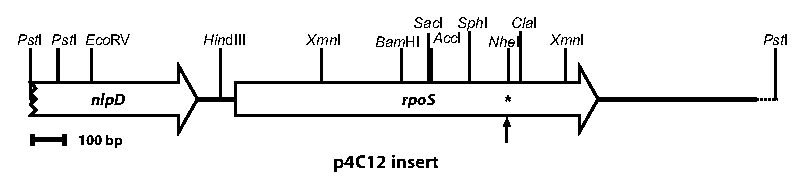
\includegraphics{figures/chap3_4c12_map}
\caption[Schematic map of plasmid p4C12]{Schematic map of plasmid
p4C12 drawn to  scale. The arrows indicate reading frames. The
broken arrow indicates partial reading frame. The dotted portion
at the end indicates the region not sequenced. Note the position
of the \emph{Nhe}I site created by a G to T transversion at
position 1324 of the sequence. The mutation results E253 to change
to an \emph{amber}. The position of the \emph{amber} is shown by
``$\ast$'' and marked with a arrow.} \label{chap3:4c12_map}
\end{figure}



\subsection{\emph{rpoS} homolog of Lz4W contains an amber}




The occurrence of the amber mutation within the reading frame of
\lzsig{} raised the possibility that the mutation might have
occurred during propagation of the plasmid p4C12 in \bact{Ec}. To
rule out this possibility, plasmids from several clones were
sequenced. It was confirmed that all the clones contain the amber
within the \e{rpoS} reading frame. The corresponding region of the
electrophoretogram is shown in Figure~\ref{chromatogram}.
Interestingly, the presence of the amber caused the creation of a
unique \emph{Nhe}I site. Taking advantage of this fact we tested
whether the amber is present in genomic sequence of Lz4W.

\begin{figure}[tbp]
\centering
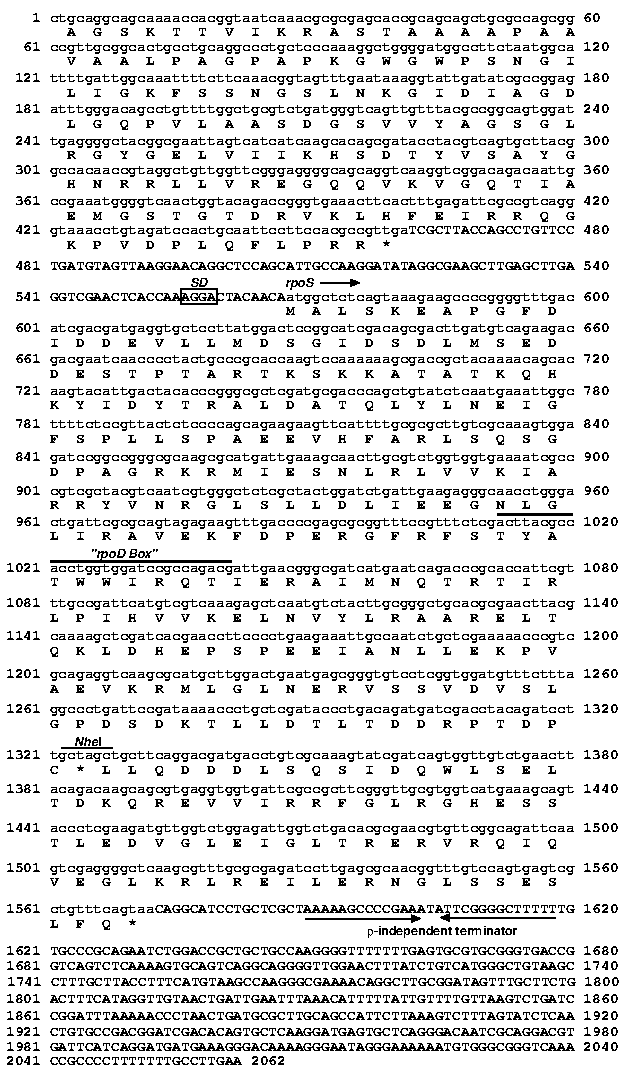
\includegraphics{figures/chap3_4c12}
\caption[\emph{rpoS} homolog of Lz4W]{The complete sequence of the
insert in plasmid p4C12 except a few terminal nucleotides. The
partial reading frame of \emph{nlpD} and the full sequence of
\emph{rpoS} with translated amino acids are shown. The reading
frames are indicated in lower case. Shine-Dalgarno sequence
(labelled SD), "\emph{rpoD} box", and $\rhoup$-independent
terminator sequence, with convergent arrows denoting the
complementary region of the hairpin loop, are indicated. Note the
presence of an amber codon in position 1324 of the sequence
(marked with $\ast$) and the resulting creation of \emph{Nhe}I
site within \emph{rpoS} reading frame. The amino acids are shown
in single letter code.} \label{chap3:4c12}
\end{figure}

The presence of the amber within \emph{rpoS} reading frame was
tested in two independent lines of Lz4W that were maintained in
our laboratory in parallel. Presence of \emph{Nhe}I site within
the reading frame would indicate the presence of amber. If
present, the \emph{Nhe}I site, upon digestion would split the
\U{$\sim$2.1}{kb} \emph{Pst}I fragment into 2 fragments with sizes
1300 and \U{740}{bp}. Lz4W genomic DNA, isolated from both the
lines of Lz4W was digested with \emph{Pst}I, and \emph{Pst}I plus
\emph{Nhe}I, and was probed with the insert from p4C12
(Figure~\ref{chap3:amber}).

\begin{figure}[tbp]
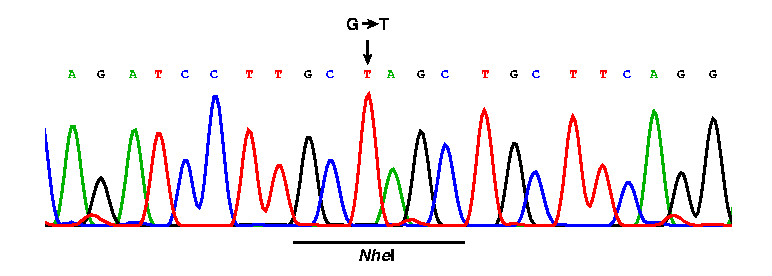
\includegraphics{figures/chap3_chromatogram.pdf}
\caption[Chromatogram of \emph{rpoS} showing the
\emph{amber}]{Portion of the chromatogram of p4C12 showing the
amber. The G to T transversion at position 1324 is marked. The
\emph{Nhe}I site created due to \emph{amber} is also shown.}
\label{chromatogram}
\end{figure}

As shown in Figure~\ref{chap3:amber} both the lines of Lz4W had
the internal \e{Nhe}I site. In \emph{Pst}I and \emph{Nhe}I double
digested DNA the \emph{rpoS} band was split into two fragments of
1300 and \U{750}{bp} in size (lanes 2 and 4 in
Figure~\ref{chap3:amber}). The residual \emph{rpoS} bands in both
these lanes was because of incomplete digestion by \emph{Nhe}I.
\begin{figure}[tbp]
\centering
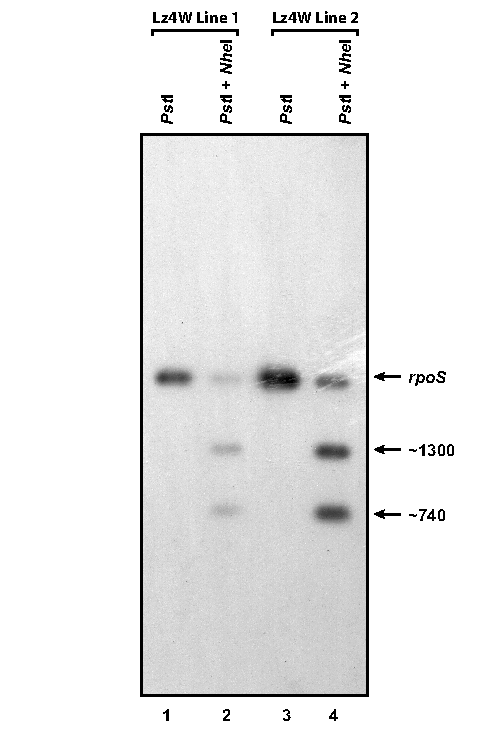
\includegraphics{figures/chap3_amber}
\caption[Presence of amber with \emph{rpoS} reading
frame]{Presence of amber within \emph{rpoS} reading frame in Lz4W
genome. Genomic DNA isolated from two independently maintained
lines of Lz4W was probed with p4C12 insert in Southern
hybridization. \emph{rpoS} band and two smaller fragments created
by \emph{Pst}I and \emph{Nhe}I double digestion is marked with
arrows. The enzymes used are indicated on top and the lane numbers
are indicated below. Lane 1, Lz4W line 1 digested with
\emph{Pst}I; lane 2, Lz4W line 1 digested with both \emph{Pst}I
and \emph{Nhe}I; lane 3, Lz4W line 2 digested with \emph{Pst}I;
lane 4, Lz4W line 2 digested with both \emph{Pst}I and
\emph{Nhe}I.} \label{chap3:amber}
\end{figure}
\subsection{Southern analysis using \emph{P. aeruginosa rpoH} as
probe}

To explore the suitability of using \emph{P. aeruginosa rpoH} gene
coding for the heat-shock $\sigmaup$ factor, $\sigmaup$\su{32}, as
heterologous probe for cloning the corresponding gene from Lz4W,
the gene was used in Southern hybridization analysis. A
\U{1.9}{kb} \emph{Sal}I--\emph{Pst}I fragment from plasmid
pRPOH5~\citep{Aramaki1996}, spanning the full-length \emph{rpoH}
of \bact{Pa} was used as heterologous probe in Southern analysis
of Lz4W genomic DNA, digested with several enzymes
(Figure~\ref{chap3:rpoh_southern}). As shown in the figure, a
\emph{Sal}I fragment of around \U{3}{kb} strongly binds to the
probe, suggesting its presence and similarity with the Lz4W gene.
The binding also suggested the feasibility of using this gene as
probe for cloning the homolog from Lz4W.

\begin{figure}[tbp]
\centering
\begin{narrow}{-1in}{0in}
\flushright
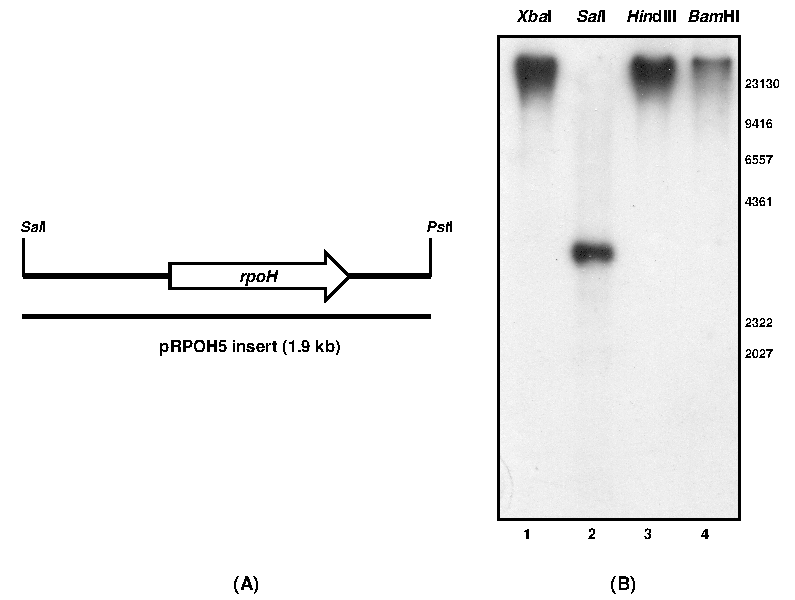
\includegraphics{figures/chap3_rpoh}
\end{narrow}
\caption[Southern analysis using \emph{P. aeruginosa rpoH}]{%
    Southern hybridization analysis using \emph{P. aeruginosa rpoH} as probe. \textbf{(A)} Schematic diagram of the probe
    used. A \U{1.9}{kb} \emph{Sal}I--\emph{Pst}I fragment from
    plasmid pRPOH5~\citep{Aramaki1996} spanning the full-length \emph{rpoH}
    of \emph{P. aeruginosa} was used to probe the genomic DNA
    of Lz4W, digested with various enzyme. The solid line below
    the map indicates the span of the probe. \textbf{(B)}
    shows the autoradiogram. Numbers along the right side
    indicate the markers in base-pairs. Approximately \mug{3} digested
    DNA was loaded in each lane. The enzymes used are indicated on the
    top of each lane and numbers below each lane show the lane
    numbers. Lane 1, \emph{Xba}I; lane 2, \emph{Sal}I; lane 3, \emph{Hin}dIII;
    lane 4, \emph{Bam}HI.}
\label{chap3:rpoh_southern}
\end{figure}



\subsection{Southern analysis using \bact{Ec} \emph{rpoA} as probe}

With similar intention to that of \e{rpoH}, \emph{E. coli}
$\alphaup$ was used as probe in Southern analysis of Lz4W genomic
DNA (\ref{chap3_fig:alpha_southern}), to examine the possibility
of using this gene to clone the homolog from Lz4W. Lz4W genomic
DNA was digested with various restriction enzymes and probed with
an \U{1.2}{kb} \emph{Xba}I fragment from the plasmid pGEMAX185
\citep{Igarashi1991}. As shown in the Figure
\ref{chap3_fig:alpha_southern}, \emph{E. coli rpoA} binds to Lz4W
genomic DNA strongly, suggesting strong sequence homology. A
\emph{Bam}HI fragment of \U{$\sim$7}{kb}, and two \emph{Sal}I
fragments, of sizes \U{$\sim$7}{kb}, and \U{$\sim$4}{kb} were
detected.

\begin{figure}[tbp]

\centering

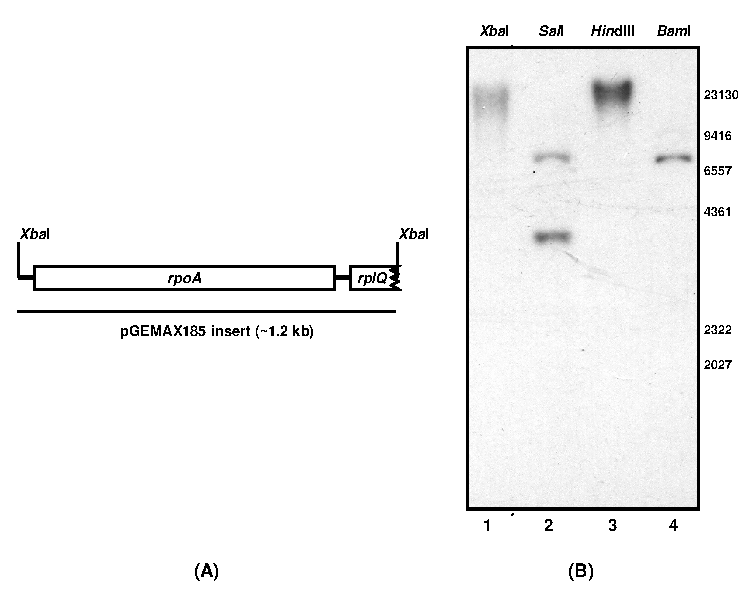
\includegraphics{figures/chap3_alpha_southern}

\caption[Southern analysis using \emph{E.coli rpoA}
probe]{Southern hybridization analysis using \emph{E. coli rpoA}
probe. \textbf{(A)} Schematic diagram of the probe used. A
\U{1.2}{kb} \emph{Xba}I fragment form plasmid pGEMAX185
\citep{Igarashi1991} was used to probe the genomic DNA from Lz4W
digested with various enzymes. The line below the map shows the
span of the probe used. \textbf{(B)} shows the autoradiogram.
Numbers along the right side indicate the markers in base-pairs.
Approximately \mug{3} digested DNA was loaded in each lane. The
enzymes used are indicated on the top of each lane and numbers
below each lane show the lane numbers. Lane 1, \emph{Xba}I; lane
2, \emph{Sal}I; lane 3, \emph{Hin}dIII; lane 4, \emph{Bam}HI.}

\label{chap3_fig:alpha_southern}

\end{figure}


\subsection{Southern analysis using \emph{rpoB} and \emph{rpoC}}

To examine whether or not \emph{E. coli} \emph{rpoB} and
\emph{rpoC} (coding for $\betaup$ and $\betaup'$ subunits
respectively, of RNA polymerase) hybridize to Lz4W genomic DNA,
genomic Southern analysis was performed using \emph{E. coli}
\emph{rpoB} and \emph{rpoC} genes
(Figure~\ref{chap3:beta_southern}). The \U{10.2}{kb}
\emph{Hin}dIII insert from the plasmid pGEMBC~\citep{Igarashi1991}
containing the full-length \emph{rpoB}, and \emph{rpoC} from
\emph{E. coli} was used as a heterologous probe in genomic
Southern hybridization. We detected very strong hybridization
signals, indicating very strong sequence conservation between
these genes.

\begin{figure}[tbp]

\centering

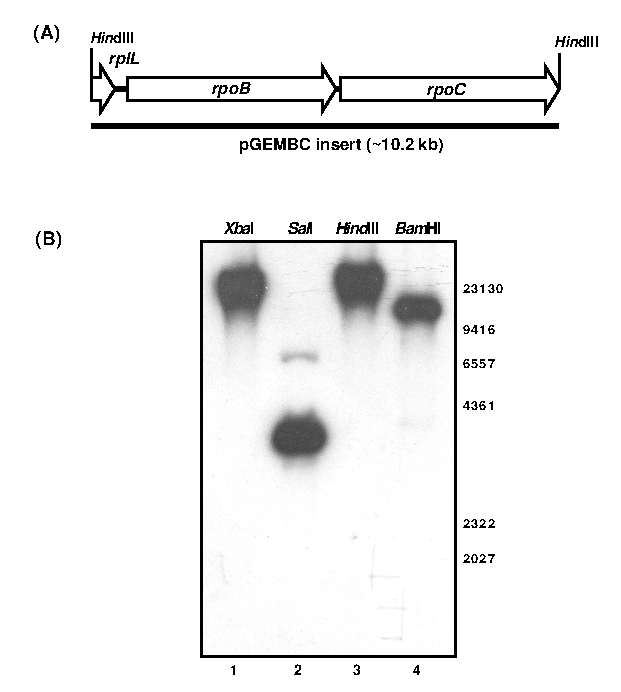
\includegraphics{figures/chap3_beta_southern}

\caption[Southern analysis using \emph{E. coli rpoB} and
\emph{rpoC}]{Southern hybridization analysis of Lz4W genomic DNA
using \emph{E. coli rpoB} and \emph{rpoC} as probe. The
\U{10.2}{kb} \emph{Hin}dIII insert from plasmid pGEMBC
\citep{Igarashi1991} was used to probe Lz4W genomic DNA digested
with various restriction enzymes. \textbf{(A)} Schematic diagram
of the probe used. The insert contained the full-length
\emph{rpoB} and \emph{rpoC} gene of \emph{E. coli} with upstream
\emph{rplL}. The solid line below the map shows the span of the
probe used. \textbf{(B)} The autoradiogram. Approximately
\mug{3--4} of digested genomic DNA was used in each lane. The
enzymes are indicated on top. The numbers along the right hand
side indicate the marker positions in base-pairs. The numbers
below mark the lanes. Lane 1, \emph{Xba}I; lane 2, \emph{Sal}I;
lane 3, \emph{Hin}dIII and lane 4, \emph{Bam}HI.}

\label{chap3:beta_southern}

\end{figure}


\section{Discussion}

$\sigmaup$ factors of proteobacteria are conserved in their
sequences, structures and functions in evolution. Several
$\sigmaup$ factors were cloned exploiting the close sequence
similarities. Traditionally, an oligomer, named ``\emph{rpoD}
box'', designed from the most conserved regions 2.3/2.4 had been
used to clone various members of $\sigmaup$\su{70} family of
$\sigmaup$ factors. Although, $\sigmaup$ factors from
Gram-positive bacteria and Gram-negative bacteria differ in their
molecular weight and overall amino acid sequence (\emph{e.g.},
\emph{B. subtilis} primary $\sigmaup$ factor is of the size
\U{43}{kDa} and \emph{E. coli} vegetative $\sigmaup$ is of the
size \U{70}{kDa}), distinct sequence similarities in several
domains enabled the cloning of $\sigmaup$ factors by heterologous
probes. Not only the primary $\sigmaup$ factors, but other members
of $\sigmaup$\su{70} family of \emph{E. coli} (\emph{rpoH},
\emph{rpoS}) are interchangeable in function across species,
enabling functional complementation by these genes.

In this study, \emph{rpoD} and \emph{rpoS} gene fragments were
amplified using degenerate PCR primers, designed from the most
conserved region of the $\sigmaup$\su{70} family. Using the
amplified fragment a partial ORF coding for \emph{rpoD} was
cloned. A full-length ORF coding for \emph{rpoS} of Lz4W was also
cloned using the amplified fragment and \bact{Pa} \emph{rpoS} gene
as probes. Both \emph{rpoD} and \emph{rpoS} homologs show strong
sequence similarities with the corresponding genes of other
pseudomonads. Interestingly, the \emph{rpoS} gene of Lz4W is
interrupted at codon 253 by an amber. The implications of this
mutation in this organism was investigated further, the results of
which are presented in subsequent chapters.

Several standards method of cloning \siga{} family members were
not successful. The attempt to clone $\sigmaup$ gene using
``\emph{rpoD} box" probe failed, in spite of it providing strong
signals in Southern hybridization. Two false positives were
detected using this probe. One of them contained \emph{trk} and
\emph{fmu} homologs of \emph{E. coli}. This clone was detected in
two independent partial genomic libraries of Lz4W. As there is no
evidence of any sequence similarity between this clone and
``\emph{rpoD} box'', there is no explanation for the reason of
strong signals detected using the oligomer. The other false
positive contained partial \emph{phoB} and \emph{pot} operon. In
this case there is prior evidence of false binding of \emph{E.
coli rpoS} probe to \emph{Bradyrhizobium japonicum
phoB}~\citep{Minder1998}.

The cloning attempt by complementation of \bact{Ec} \e{rpoD}
mutant UQ285 was not successful. Among several possible
explanations mentioned earlier, the possibility of a toxic effect
of Lz4W \e{rpoD}, when cloned in \bact{Ec} merits attention. As
shown, the gene, when fragmented, could be readily cloned in
\emph{E. coli}, implicating a toxic effect of the full-length
gene. The cloned part of \emph{rpoD} shows strong sequence
conservation with \emph{rpoD} of other pseudomonads.

Inability of Lz4W \emph{rpoS} to complement \bact{Ec} \e{rpoS}
mutant ZK918 could be easily explained because of the presence of
amber within the \emph{rpoS} reading frame of Lz4W. In later
Chapters we provide evidence that this \emph{rpoS} allele is
unable to induce \emph{bolAp1} promoter to such as extent, so as
to be able to distinguish cells harboring \emph{rpoS} from the
background.

Additionally, Lz4W $\alphaup$, $\betaup$, $\betaup'$, and
$\sigmaup$\su{H}, coded by \emph{rpoA}, \emph{rpoB}, \emph{rpoC}
and \emph{rpoH} respectively, are  similar to the respective
homologs in other bacteria, at the primary sequence level. This
conclusion is based on the strong signals detected in Southern
hybridization analysis of Lz4W genomic DNA with heterologous
probes, enabling the future cloning of these subunits by
heterologous probes, a possibility.\ding{45}
